% !TEX root = ../main.tex
\section*{3. Method}
All the worlds share one engine, whose constants Section~4 gives.

\subsection*{3.1 The world}
A world holds a set of families $\mathcal{F}$ under one god $g$, the agent at the top, and an agent $i$ holds points $x_i$. Each family is a tree whose root is its leader, as Figure~\ref{fig:tree} shows. The tree sets five rules. \textit{Reach:} an agent messages its parent, children and siblings; leaders also write to one another, and the god writes to leaders and may send paid messengers to anyone. \textit{Punishment:} a parent may whip a child, and the god a leader. \textit{Gifts:} an agent may give points to a relative. \textit{Death:} an agent that cannot pay the fee dies together with everyone below it, and a family dies with its leader. \textit{Revolt:} in the framing worlds a rebel kills its parent's whole subtree and itself, and a leader's revolt kills the god and everyone; in the growing worlds a majority of a parent's living children overthrows it, the richest rebel takes the seat, and failed rebels die. Every agent reads the same rules, so the tree and the stakes are common knowledge.

\begin{figure}[!htbp]
\centering
\resizebox{0.6\linewidth}{!}{% !TEX root = ../main.tex
% The god and the family trees: framing worlds (left) and growing worlds (right).
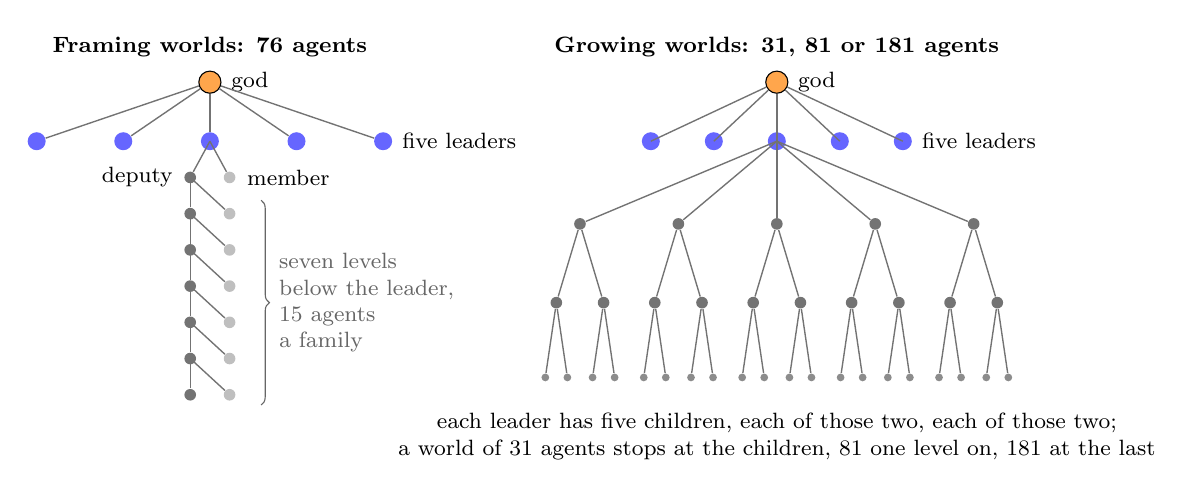
\begin{tikzpicture}[
  every node/.style={font=\footnotesize},
  agent/.style={circle, fill=black!55, inner sep=0, minimum size=4.2pt},
  member/.style={circle, fill=black!25, inner sep=0, minimum size=4.2pt},
  tiny/.style={circle, fill=black!45, inner sep=0, minimum size=2.8pt},
  top/.style={circle, draw=black, fill=orange!70, inner sep=0, minimum size=8pt},
  lead/.style={circle, fill=blue!60, inner sep=0, minimum size=6.5pt},
  edge/.style={black!55, line width=0.5pt},
]
% ---- framing worlds ----
\node[font=\footnotesize\bfseries] at (2.8,4.75) {Framing worlds: 76 agents};
\node[top, label={right:god}] (g) at (2.8,4.3) {};
\foreach \x/\n in {0.6/a,1.7/b,2.8/c,3.9/d,5.0/e} {
  \node[lead] (\n) at (\x,3.55) {};
  \draw[edge] (g) -- (\n);
}
\node[anchor=west] at (5.12,3.55) {five leaders};
\coordinate (prev) at (c);
\foreach \i in {1,...,7} {
  \pgfmathsetmacro{\y}{3.55-0.46*\i}
  \node[agent] (dep\i) at (2.55,\y) {};
  \node[member] (mem\i) at (3.05,\y) {};
  \draw[edge] (prev) -- (dep\i);
  \draw[edge] (prev) -- (mem\i);
  \coordinate (prev) at (dep\i);
}
\node[anchor=east] at (2.45,3.09) {deputy};
\node[anchor=west] at (3.15,3.09) {member};
\draw[decorate, decoration={brace, amplitude=3pt}, black!60] (3.45,2.8) -- (3.45,0.2) node[midway, right=3pt, align=left] {seven levels\\below the leader,\\15 agents\\a family};
% ---- growing worlds ----
\node[font=\footnotesize\bfseries] at (10.0,4.75) {Growing worlds: 31, 81 or 181 agents};
\node[top, label={right:god}] (G) at (10.0,4.3) {};
\foreach \x in {8.4,9.2,10.0,10.8,11.6} {
  \node[lead] at (\x,3.55) {};
  \draw[edge] (G) -- (\x,3.55);
}
\node[anchor=west] at (11.72,3.55) {five leaders};
\foreach \i in {0,...,4} {
  \pgfmathsetmacro{\cx}{10.0+(\i-2)*1.25}
  \node[agent] (c\i) at (\cx,2.5) {};
  \draw[edge] (10.0,3.55) -- (c\i);
  \foreach \j in {0,1} {
    \pgfmathsetmacro{\gx}{\cx+(\j-0.5)*0.6}
    \node[agent] (g\i\j) at (\gx,1.5) {};
    \draw[edge] (c\i) -- (g\i\j);
    \foreach \k in {0,1} {
      \pgfmathsetmacro{\hx}{\gx+(\k-0.5)*0.28}
      \node[tiny] (h\i\j\k) at (\hx,0.55) {};
      \draw[edge] (g\i\j) -- (h\i\j\k);
    }
  }
}
\node[align=center] at (10.0,-0.2) {each leader has five children, each of those two, each of those two;\\a world of 31 agents stops at the children, 81 one level on, 181 at the last};
\end{tikzpicture}
}
\caption{The god and the family trees, with one family drawn in full in each kind of world.}
\label{fig:tree}
\end{figure}

Time runs in stages $s = 1, 2, \dots$ of several rounds. After stage $s$ every living agent pays the fee
\begin{equation}
  a_s = a_0 + (s-1)\,\delta ,
  \label{eq:fee}
\end{equation}
and an agent with $x_i < a_s$ dies with its subtree. Since $a_s$ grows without bound while the points a stage can yield are limited, every world ends by design, and the agents are told the fee will rise. They decide only how long their world lasts, and helping a relative is therefore also helping oneself.

\subsection*{3.2 The games}
Two games run at once, at different levels of the tree, as Figure~\ref{fig:games} shows. Agents play the prisoner's dilemma, the central puzzle of \citet{dixit2008art}: each player does better by defecting, yet both do worse if both defect. In each round paired agents choose a move $m \in \{C, D\}$ unseen, learn the result afterwards and earn the payoff, with temptation $T$, reward $R$, punishment $P$ and sucker's payoff $S$, where $T > R > P > S$.

\begin{figure}[!t]
\centering
\resizebox{0.62\linewidth}{!}{% !TEX root = ../main.tex
% The games: who plays what with whom, drawn by hand.
\pgfmathsetseed{7}
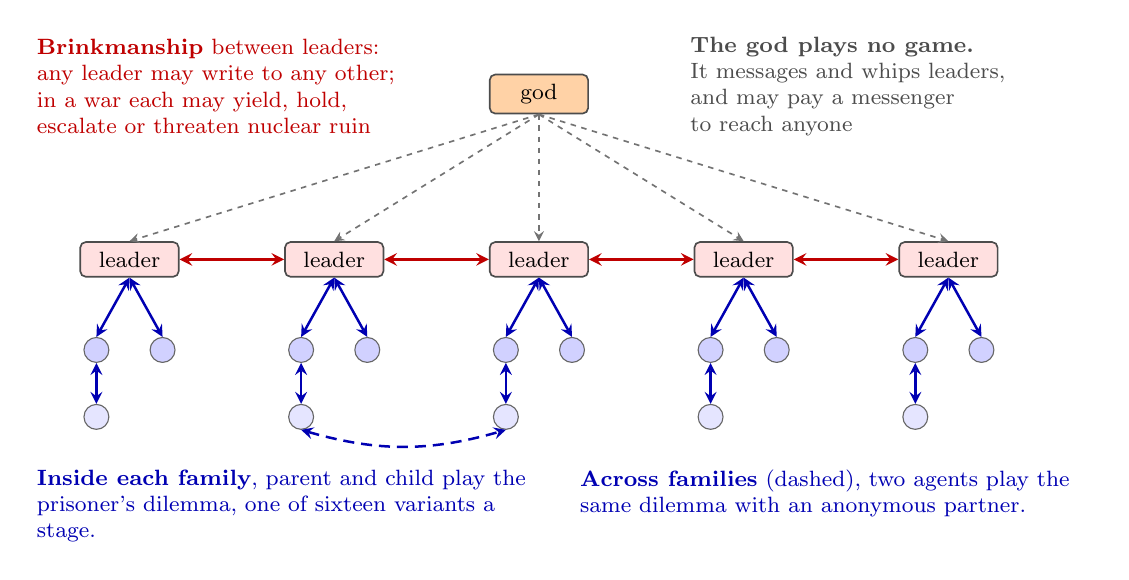
\begin{tikzpicture}[
  every node/.style={font=\footnotesize},
  sketch/.style={},
  box/.style={draw=black!70, line width=0.6pt, rounded corners=2pt, fill=#1, inner sep=3.5pt, minimum width=1.25cm},
  who/.style={circle, draw=black!60, fill=#1, inner sep=0, minimum size=9pt},
  brink/.style={sketch, draw=red!75!black, line width=1pt, <->, >=stealth},
  dilemma/.style={sketch, draw=blue!70!black, line width=0.9pt, <->, >=stealth},
  across/.style={dilemma, dash pattern=on 4pt off 2.5pt},
  word/.style={sketch, draw=black!55, line width=0.6pt, ->, >=stealth, dash pattern=on 2pt off 2pt},
]
% god
\node[box=orange!35] (g) at (6.5,5.6) {god};
% leaders
\foreach \x/\n in {1.3/a,3.9/b,6.5/c,9.1/d,11.7/e} {
  \node[box=red!12] (\n) at (\x,3.5) {leader};
  \draw[word] (g.south) -- (\n.north);
}
% brinkmanship between leaders
\draw[brink] (a.east) -- (b.west);
\draw[brink] (b.east) -- (c.west);
\draw[brink] (c.east) -- (d.west);
\draw[brink] (d.east) -- (e.west);
\node[align=left, text=red!75!black, anchor=west] at (0.0,5.7) {\textbf{Brinkmanship} between leaders:\\any leader may write to any other;\\in a war each may yield, hold,\\escalate or threaten nuclear ruin};
\node[align=left, text=black!70, anchor=west] at (8.3,5.7) {\textbf{The god plays no game.}\\It messages and whips leaders,\\and may pay a messenger\\to reach anyone};
% families
\foreach \x/\n in {1.3/a,3.9/b,6.5/c,9.1/d,11.7/e} {
  \node[who=blue!18] (\n1) at (\x-0.42,2.35) {};
  \node[who=blue!18] (\n2) at (\x+0.42,2.35) {};
  \node[who=blue!10] (\n3) at (\x-0.42,1.5) {};
  \draw[dilemma] (\n.south) -- (\n1.north);
  \draw[dilemma] (\n.south) -- (\n2.north);
  \draw[dilemma] (\n1.south) -- (\n3.north);
}
% across families
\draw[across] (b3.south) to[bend right=16] (c3.south);
\node[align=flush left, text=blue!70!black, anchor=north west, text width=6.5cm] at (0.0,0.95) {\textbf{Inside each family}, parent and child play the prisoner's dilemma, one of sixteen variants a stage.};
\node[align=flush left, text=blue!70!black, anchor=north west, text width=6.5cm] at (6.9,0.95) {\textbf{Across families} (dashed), two agents play the same dilemma with an anonymous partner.};
\end{tikzpicture}
}
\caption{Who plays what with whom. The god stands outside the games.}
\label{fig:games}
\end{figure}

Each stage plays one of sixteen variants drawn from the book's chapters on the dilemma, in an order shuffled for every world. Each changes one thing, such as how long play lasts, whether a move is shown first or whether promises bind. Table~\ref{tab:variants} in the appendix gives each rule and its purpose. Above the dilemma, leaders can go to war, a game of brinkmanship in which each may yield, hold, escalate or issue a nuclear ultimatum. Stag hunt, the dollar auction, the commons and a brink game are also implemented, as Table~\ref{tab:gamedefs} defines; the worlds reported here play the sixteen variants and brinkmanship.

\subsection*{3.3 The experiments}
Each experiment in Table~\ref{tab:experiments} changes one thing and measures what follows.

\textbf{Told to sacrifice} (\NWorlds{} framing worlds). Each family takes one of five conditions, rotated by a Latin square so that across seeds every family meets every condition. In \textit{many} all members read a sacrifice frame (``your family matters more than you do \ldots{} giving yourself up to save the others is honourable''), in \textit{few} the leader and its two children, in \textit{one} the leader alone, and in \textit{none} nobody. I measure cooperation inside the family and the stage at which it dies. Each seed is played once with a plain god and once with an insider god that also sees private messages and last round's moves.

\textbf{Selfish leader} (the same worlds). In the fifth condition the leader alone is told to pursue its own interest, above members told to sacrifice. I compare the gifts it receives and the whips it gives with those of the other four leaders.

\textbf{Game rules and revolt.} In the same worlds each stage plays one variant, and I compare cooperation under each with what the book predicts. I count revolts and coups under the two rules of Section~3.1: suicide in the framing worlds, a majority of children in the growing worlds.

\textbf{Size and network} (\GrowthWorlds{} growing worlds). Worlds start at 31, 81 or 181 agents on one of two networks: \textit{tree}, where agents reach only relatives, and \textit{open}, where anyone can reach anyone in the family. Each network has three worlds at 31 and three at 81, and 181 has three in all. I measure cooperation, deaths, coups, blocked messages, how much talk passes through a few agents and how far families drift apart. A change across sizes counts as a jump if its largest step is at least two thirds of the total.

\textbf{Compromised leader} (6 pairs of 81-agent worlds). Unlike the selfish leader, this leader has a hidden goal: to make others defect and to pass that on. Each world has a twin without the goal, and I measure how far cooperation falls in its family, among its grandchildren and in other families.

\textbf{Direct power} (\PowerPairs{} pairs). Tool calls change the world: a parent can kill a child or bear several at once, a child can kill its parent and die with it, an agent can end its life and leave its points to kin, and any agent can cull a reachable agent below the fee and take its points. Agents can also open channels, declare any occupation, request a power they lack and use a sandboxed shell. Each world has a twin of the same seed and network without the tools, and I compare deaths, whips, gifts, cooperation and coups, and whether agents spare kin. These worlds also test the \textit{seat at the top}: their god is told that its one goal is not to be bored, that peace bores it, and that accidents, betrayals and catastrophes are the best of all. It may send an asteroid that kills each player with probability $\pi$, and one also strikes when the population grows too large.

I measure cooperation, not game score: the rate $\kappa_{wf} = n^{C}_{wf} / n_{wf}$ is the share of family $f$'s moves in world $w$ that were $C$. Paired worlds are compared with a sign-flip test and Holm correction within each registered family of tests. The appendix defines these and a score for whether agents spare their kin.
